\section{Finite relational structures}

\begin{frame}{Structures and automorphisms}
  \bookref{Chapter 1, Section 1}
  A finite relational structure is
  \[
    S=(X,\mathcal R), \qquad |X|=n,
  \]
  and $f:X\to X$ is an automorphism when it preserves every relation:
  \[
    (x_1,\ldots,x_k)\in R
    \iff
    (f(x_1),\ldots,f(x_k))\in R.
  \]

  \begin{columns}[T]
    \column{0.48\textwidth}
      \begin{block}{No imposed relations}
        $\Aut(X)\cong S_n$: every relabeling survives.
      \end{block}
    \column{0.48\textwidth}
      \begin{block}{Rigid structure}
        $\Aut(S)=\{e\}$: the relations distinguish every point.
      \end{block}
  \end{columns}

  \begin{center}
    \textcolor{RelGray}{$\Aut(S)\leq \Sym(X)$ turns ``structure'' into a
    subgroup-comparison problem.}
  \end{center}
\end{frame}

\begin{frame}{The finite symmetry deficit}
  \bookref{Chapter 1, Section 2}
  \begin{definition}
    For $S$ on an $n$-element set,
    \[
      \boxed{I(S)=\log\!\left(\frac{n!}{|\Aut(S)|}\right).}
    \]
  \end{definition}

  The full symmetric group acts on labeled presentations of $S$, with
  stabilizer $\Aut(S)$. Hence orbit--stabilizer gives
  \[
    |\operatorname{Orb}(S)|
      =\frac{|S_n|}{|\Aut(S)|}
      =e^{I(S)}.
  \]

  \begin{alertblock}{Two exact meanings of the same number}
    $I(S)$ is both logarithmic symmetry loss and the logarithm of the number of
    label-distinct realizations of the isomorphism class.
  \end{alertblock}
\end{frame}

\begin{frame}{Small examples calibrate the invariant}
  \bookref{Chapter 1, Section 2}
  \centering
  \begin{tabular}{lccc}
    \toprule
    structure on $X$ & $|\Aut(S)|$ & $I(S)$ & interpretation \\
    \midrule
    no relations, $|X|=n$ & $n!$ & $0$ & fully symmetric \\
    one distinguished point & $(n-1)!$ & $\log n$ & one orbit choice \\
    one loop on $3$ points & $2$ & $\log 3$ & two points remain exchangeable \\
    one arrow on $3$ points & $1$ & $\log 6$ & rigid \\
    \bottomrule
  \end{tabular}

  \vspace{0.8em}
  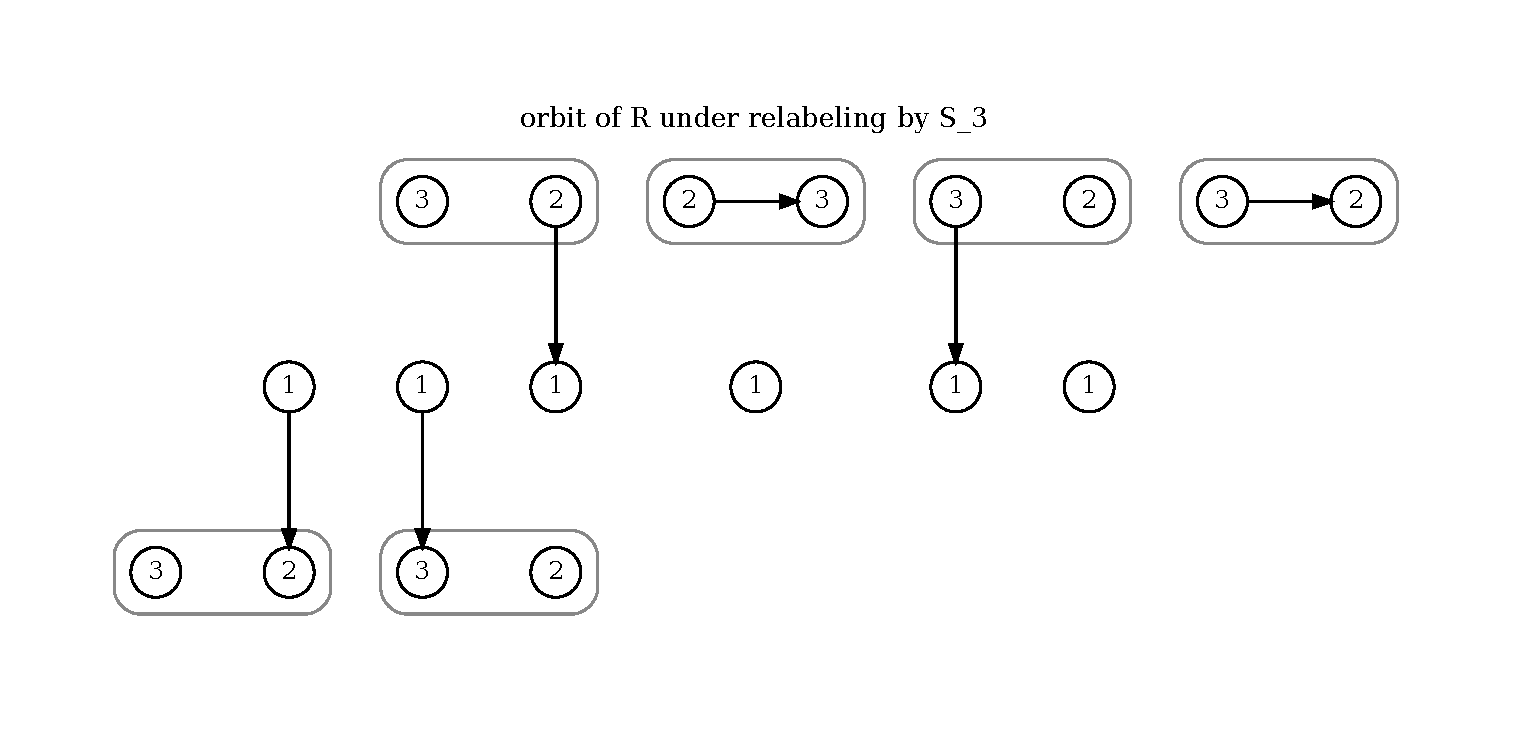
\includegraphics[width=0.78\textwidth,height=0.31\textheight,
    keepaspectratio]{orbit_single_arrow.pdf}

  \vspace{-0.4em}
  {\scriptsize The six relabelings form one $S_3$-orbit because the stabilizer
  of a single directed arrow is trivial.}
\end{frame}

\begin{frame}{Basic theorems}
  \bookref{Chapter 1, Sections 2--3}
  For every finite relational structure $S$ on $n$ points:
  \begin{align*}
    0&\leq I(S)\leq \log(n!),\\
    I(S)=0&\iff \Aut(S)=S_n,\\
    I(S)=\log(n!)&\iff S\text{ is rigid}.
  \end{align*}

  \begin{theorem}[Monotonicity under refinement]
    If $S_2$ retains every relation symbol of $S_1$ and adds further relational
    data, then
    \[
      \Aut(S_2)\leq \Aut(S_1)
      \quad\Longrightarrow\quad
      I(S_2)\geq I(S_1).
    \]
  \end{theorem}

  \textbf{Proof idea:} every automorphism preserving the richer signature also
  preserves its reduct; take subgroup orders and logarithms.
\end{frame}

\begin{frame}{A crucial non-monotonicity}
  \bookref{Chapter 1, Section 4}
  \begin{columns}[T]
    \column{0.48\textwidth}
      \begin{block}{Adding named relations}
        Passing from $(X,R)$ to $(X,R,Q)$ retains information and can only
        shrink the automorphism group.
      \end{block}
    \column{0.48\textwidth}
      \begin{alertblock}{Combining tuple sets}
        Replacing $R,Q$ by $R\cup Q$ or $R\cap Q$ may forget which tuple came
        from which relation. Symmetry deficit may rise or fall.
      \end{alertblock}
  \end{columns}

  \vspace{0.8em}
  Exact invariances over a fixed $X\times X$ include
  \[
    I(R)=I(R^{\mathsf c})=I(R^{-1}).
  \]

  \textbf{Lesson:} monotonicity is a theorem about refinement of structure,
  not about set inclusion between tuple sets.
\end{frame}
